\documentclass[
  bibliography=totoc,     % Literatur im Inhaltsverzeichnis
  captions=tableheading,  % Tabellenüberschriften
  titlepage=firstiscover, % Titelseite ist Deckblatt
]{scrartcl}

% Paket float verbessern
\usepackage{scrhack}

% Warnung, falls nochmal kompiliert werden muss
\usepackage[aux]{rerunfilecheck}

% unverzichtbare Mathe-Befehle
\usepackage{amsmath}
% viele Mathe-Symbole
\usepackage{amssymb}
% Erweiterungen für amsmath
\usepackage{mathtools}

% Fonteinstellungen
\usepackage{fontspec}
% Latin Modern Fonts werden automatisch geladen
% Alternativ:
%\setromanfont{Libertinus Serif}
%\setsansfont{Libertinus Sans}
%\setmonofont{Libertinus Mono}
\recalctypearea % Wenn man andere Schriftarten gesetzt hat,
% sollte man das Seiten-Layout neu berechnen lassen

% deutsche Spracheinstellungen
\usepackage{polyglossia}
\setmainlanguage{german}


\usepackage[
  math-style=ISO,    % ┐
  bold-style=ISO,    % │
  sans-style=italic, % │ ISO-Standard folgen
  nabla=upright,     % │
  partial=upright,   % ┘
  warnings-off={           % ┐
    mathtools-colon,       % │ unnötige Warnungen ausschalten
    mathtools-overbracket, % │
},                       % ┘
]{unicode-math}

% traditionelle Fonts für Mathematik
\setmathfont{Latin Modern Math}
% Alternativ:
%\setmathfont{Libertinus Math}

\setmathfont{XITS Math}[range={scr, bfscr}]
\setmathfont{XITS Math}[range={cal, bfcal}, StylisticSet=1]

% Zahlen und Einheiten
\usepackage[
locale=DE,                   % deutsche Einstellungen
separate-uncertainty=true,   % immer Fehler mit \pm
per-mode=symbol-or-fraction, % / in inline math, fraction in display math
]{siunitx}

% chemische Formeln
\usepackage[
version=4,
math-greek=default, % ┐ mit unicode-math zusammenarbeiten
text-greek=default, % ┘
]{mhchem}

% richtige Anführungszeichen
\usepackage[autostyle]{csquotes}

% schöne Brüche im Text
\usepackage{xfrac}

% Standardplatzierung für Floats einstellen
\usepackage{float}
\floatplacement{figure}{htbp}
\floatplacement{table}{htbp}

% Floats innerhalb einer Section halten
\usepackage[
section, % Floats innerhalb der Section halten
below,   % unterhalb der Section aber auf der selben Seite ist ok
]{placeins}

% Seite drehen für breite Tabellen: landscape Umgebung
\usepackage{pdflscape}

% Captions schöner machen.
\usepackage[
  labelfont=bf,        % Tabelle x: Abbildung y: ist jetzt fett
  font=small,          % Schrift etwas kleiner als Dokument
  width=0.9\textwidth, % maximale Breite einer Caption schmaler
]{caption}
% subfigure, subtable, subref
\usepackage{subcaption}

% Grafiken können eingebunden werden
\usepackage{graphicx}
% größere Variation von Dateinamen möglich
\usepackage{grffile}

% schöne Tabellen
\usepackage{booktabs}

% Verbesserungen am Schriftbild
\usepackage{microtype}

% Literaturverzeichnis
\usepackage[style=alphabetic,]{biblatex}
% Quellendatenbank
\addbibresource{lit.bib}
\addbibresource{programme.bib}

% Hyperlinks im Dokument
\usepackage[
  unicode,        % Unicode in PDF-Attributen erlauben
  pdfusetitle,    % Titel, Autoren und Datum als PDF-Attribute
  pdfcreator={},  % ┐ PDF-Attribute säubern
  pdfproducer={}, % ┘
]{hyperref}
% erweiterte Bookmarks im PDF
\usepackage{bookmark}

% Trennung von Wörtern mit Strichen
\usepackage[shortcuts]{extdash}

\title{US3: Doppler-Sonographie}
\author{
  Simon Schulte
  \texorpdfstring{
    \\
    \href{mailto:simon.schulte@udo.edu}{simon.schulte@udo.edu}
  }{}
  \texorpdfstring{\and}{, }
  Tim Sedlaczek
  \texorpdfstring{
    \\
    \href{mailto:tim.sedlaczek@udo.edu}{tim.sedlaczek@udo.edu}
  }{}
}
\publishers{TU Dortmund – Fakultät Physik}

\date{Durchführung: 27.06.2017\\
      Abgabe: 04.07.2017}


\begin{document}

\maketitle
\thispagestyle{empty}
\tableofcontents
\newpage
\setcounter{page}{1}
\section{Zielsetzung}
\label{sec:zielsetzung}
Bei diesem Versuch wird das Verhalten von Rohrströmungen mit Ultraschall untersucht.
\section{Theorie}
\label{sec:theorie}
Als Ultraschall werden Schallwellen mit Frequenzen zwischen $\SI{20}{\kilo\hertz}$
und $\SI{1}{\giga\hertz}$ bezeichnet. Diese Frequenzen liegen oberhalb von dem,
was Menschen hören können. Für die Erzeugung dieser Schallwellen wird der
piezo-elektrische Effekt verwendet. Dabei wird ein geeigneter Kristall
elektrisch zu Schwingungen angeregt. Gleichzeitig kann die Resonanz eines solchen
Kristalls für die Messung von entsprechend hoch frequenten Schallwellen verwendet
werden. Bei dem Versuch wird, zur Messung der Geschwindigkeit der Strömung,
der Doppler-Effekt ausgenutzt. Durch die Geschwindigkeit der Strömung wird die
Frequenz der Welle verändert und die Differenz der Frequenzen kann zur Bestimmung
der Geschwindigkeiten verwendet werden.
Die Differenz der Frequenzen ergibt sich nach:
\begin{equation}
  \Delta \nu = 2 \nu_{0} \frac{v}{c} \cos \left( \alpha \right).
  \label{eqn:freqdiff}
\end{equation}
Dabei ist $\nu_{0}$ die ursprüngliche Frequenz, $v$ die Geschwindigkeit der
Strömung, $c$ die Schallgeschwindigkeit der Flüssigkeit und $\alpha$ der Winkel,
in dem die Schallwelle auf die Röhre trifft.
Demnach lässt sich die Geschwindigkeit nach
\begin{equation}
  v = \frac{\Delta \nu \cdot c}{2 \nu_{0} \cos \left( \alpha \right)}
  \label{eqn:geschw}
\end{equation}
bestimmen.\\

\noindent
Um reproduzierbare Winkel verwenden zu können und um die Ultraschall-Sonde besser
an die Röhren koppeln zu können werden bei dem Versuch Acryl-Prismen verwendet.
Wegen Brechung entsprechen die vorgegebenen Prismenwinkel nicht den für die
Bestimmung der Geschwindigkeit nötigen Dopplerwinkeln. Diese lassen sich jedoch
nach
\begin{equation}
  \alpha = \SI{90}{\degree} - \arcsin \left( \sin \left( \theta \right) \cdot \frac{c_\mathup{L}}{c_\mathup{P}} \right)
  \label{eqn:dopplerwinkel}
\end{equation}
berechnen. Dabei ist $c_\mathup{L}$ die Schallgeschwindigkeit der Flüssigkeit und
$c_\mathup{P}$ die von Acryl.
\clearpage
\section{Durchführung}
\label{sec:durchführung}
\subsection{Versuchsaufbau}
\label{sec:aufbau}
Der Aufbau besteht aus einer Schleife aus Silikonröhren, welche an eine
Zentrifugalpumpe angeschlossen ist. Sie ist zudem mit einer Phantomflüssigkeit
aus Wasser, Glycerin und Glaskugeln gefüllt. In der Schleife befinden sich drei
Abschnitte mit unterschiedlichen Durchmessern. An ihnen wird später die
Strömungsgeschwindigkeit gemessen. Für die Mesungen wird eine $\SI{2}{\mega\hertz}$-Sonde
verwendet, welche gleichzeitig als Sender und Empfänger dient. Das Signal wird
dann an einem PC ausgewerte, welcher dann die Differenz der Frequenzen anzeigt.
Zur Kopplung zwischen Sonde und Röhre werden, wie bereits erwähnt, Acryl-Prismen
verwendet. Diese liegen in drei Varianten vor, welche an die verschiedenen Durchmesser
der Röhren angepasst sind. Zusätzlich wird ein Ultraschall-Kopplungsgel verwendet.
In Abbildung \ref{fig:prisma} ist ein Acryl-Prisma mit den drei Prismenwinkeln
zu sehen.
\begin{figure}[H]
  \centering
  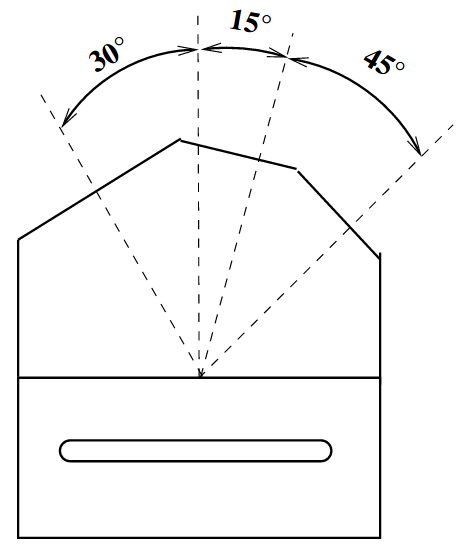
\includegraphics[width=0.3\textwidth]{prisma.png}
  \caption{Querschnitt eines Prismas. \cite{anleitung}}
  \label{fig:prisma}
\end{figure}
\noindent
Für die Phantomflüssigkeit, die Prismen und die Röhren sind die in Tabelle \ref{tab:vorgaben}
stehenden Werte gegeben.
\begin{table}
  \centering
  \caption{Technische Vorgaben.}
  \label{tab:vorgaben}
  \sisetup{table-format=2.0}
  \begin{tabular}{S S S}
    \toprule
    \text{Phantomflüssigkeit} & \SI{1.15}{\gram\per\cubic\centi\meter} & \text{Dichte} $\rho$ \\
                              & \SI{1800}{\meter\per\second} & \text{Schallgeschwindigkeit} $c_\mathup{L}$ \\
                              & \SI{12}{\milli\pascal\second} & \text{Viskosität} $\eta$ \\
    \text{Prismen} & \SI{2700}{\meter\per\second} & \text{Schallgeschwindigkeit} $c_\mathup{P}$ \\
                   & \SI{30.7}{\milli\meter} & \text{Länge der Vorlaufstrecke} $l$ \\
    \text{Röhren} & \text{Innendurchmesser} & \text{Außendurchmesser} \\
    1             & \SI{7}{\milli\meter} & \SI{10}{\milli\meter} \\
    2             & \SI{10}{\milli\meter} & \SI{15}{\milli\meter} \\
    3             & \SI{16}{\milli\meter} & \SI{20}{\milli\meter} \\
    \bottomrule
  \end{tabular}
\end{table}
\clearpage
\subsection{Versuchsablauf}
\label{sec:ablauf}
Zuerst werden verschiedene Strömungsgeschwindigkeiten bestimmt.
Dazu werden für die drei Röhren, mit den drei Prismenwinkeln, für fünf verschiedene
Pumpleistungen $\left( \SI{30}{\percent}, \SI{40}{\percent}, \SI{50}{\percent}, \SI{60}{\percent}, \SI{70}{\percent} \right)$
die durch den Doppler-Effekt entstehenden Frequenzdifferenzen gemessen.
Es werden also 45 Messwerte genommen. Für diese Geschwindigkeitsmessung
ist am Ultraschallgenerator das Sample Volume auf Large zu stellen. Aus
den Differenzen wird dann die Strömungsgeschwindigkeit bestimmt.\\

\noindent
Im zweiten Teil des Versuchs wird das Strömungsprofil der mittleren/zweiten Röhre
$\left( \SI{10}{\milli\meter} \; \text{Innendurchmesser} \right)$ unter zwei
verschiedenen Pumpleistungen $\left( \SI{45.2}{\percent}, \SI{70}{\percent} \right)$
vermessen. An dem Prisma wird dabei immer der Winkel $\SI{15}{\degree}$ verwendet.
Zum Einstellen der Messtiefe wird an dem Generator das Sample Volume auf Small
gestellt. Anschließend wird für Messtiefen von $\SI{12}{\micro\second}$ bis $\SI{19.5}{\micro\second}$
in $\SI{0.5}{\micro\second}$ Schritten die Frequenzdifferenz und die Streuintensität
gemessen.
\clearpage
\section{Auswertung}
\subsection{Bestimmung der Strömungsgeschwindigkeit für die Dopplerwinkel.}
Um die Strömungsgeschwindigkeit zu bestimmmen, wird \eqref{eqn:geschw} genutzt.
Mit \eqref{eqn:dopplerwinkel} folgt für die Dopplerwinkel $\alpha$
\begin{table}
  \centering
  \begin{tabular}{c c}
    \toprule
    $\theta$ & $\alpha$ \\
    \midrule
    15° & 80.1° \\
    30° & 70.5° \\
    60° & 54.7° \\
    \bottomrule
  \end{tabular}
  \caption{Dopplerwinkel $\alpha$ zu den vordefinierten Einfallswinkeln
  $\theta$.}
  \label{tab:1}
\end{table}
mit $c_L = \SI{1800}{\meter\per\second}$ und $c_P =
\SI{2700}{\meter\per\second}$.
Damit folgen die Ergebnisse für die drei Dopplerwinkel mit $\nu_0 =
\SI{2}{\mega\hertz}$
und $c = \SI{1800}{\meter\per\second}$ mit dem jeweils passendem Diagramm.

\begin{figure}
    \centering
      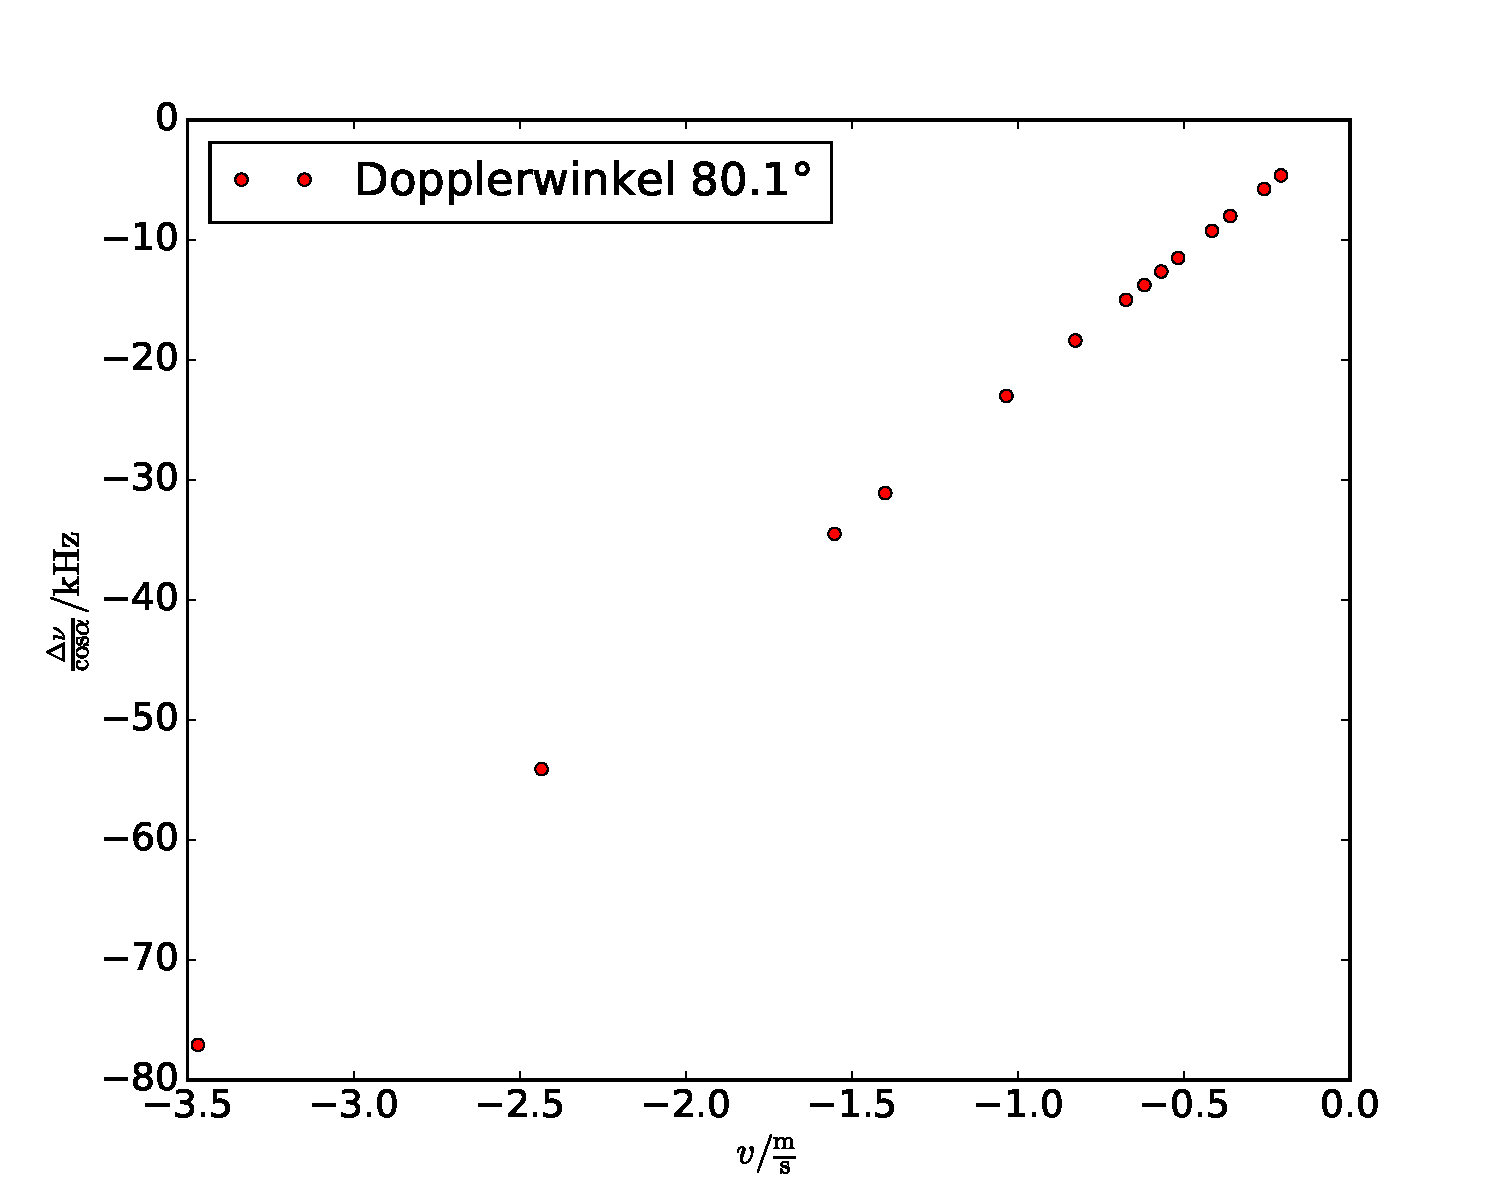
\includegraphics[width=0.8\textwidth]{a15.pdf}
      \caption{Die Frequenzverschiebung geteilt durch den cos des
      Dopplerwinkels 80.1° aufgetragen gegen die Geschwindigkeit.}
      \label{fig:1}
  \end{figure}
 \begin{table}
    \centering
    \begin{tabular}{c c c c}
      \toprule
      Pumpleistung / $\%$ & $\symup{\Delta} \nu$ / $\si{\hertz}$ & $v$ /
      \si{\meter\per\second} & Rohrdicke $\si{\milli\meter}$ \\
      \midrule
      30 & 49 & 0.21  & 16\\
      40 & 61 & 0.26  & 16\\
      50 & 98 & 0.42  & 16\\
      60 & 122 & 0.52  & 16\\
      70 & 146 & 0.62  & 16\\
      30 & 85 & 0.36  & 10\\
      40 & 134 & 0.57  & 10\\
      50 & 195 & 0.83  & 10\\
      60 & 244 & 1.04 & 10\\
      70 & 330 & 1.40 & 10\\
      30 & 159 & 0.67  & 7\\
      40 & 244 & 1.04 & 7\\
      50 & 366 & 1.56 & 7\\
      60 & 574 & 2.43 & 7\\
      70 & 818 & 3.47 & 7\\
      \bottomrule
    \end{tabular}
    \caption{Die Pumpleistung, die Frequenzverschiebung (aus den Messungen) und
    die Geschwindigkeit aus \eqref{eqn:geschw} berechnet für einen Einfallswinkel
    von 15°.}
    \label{tab:2}
  \end{table}

      \begin{figure}
      \centering
        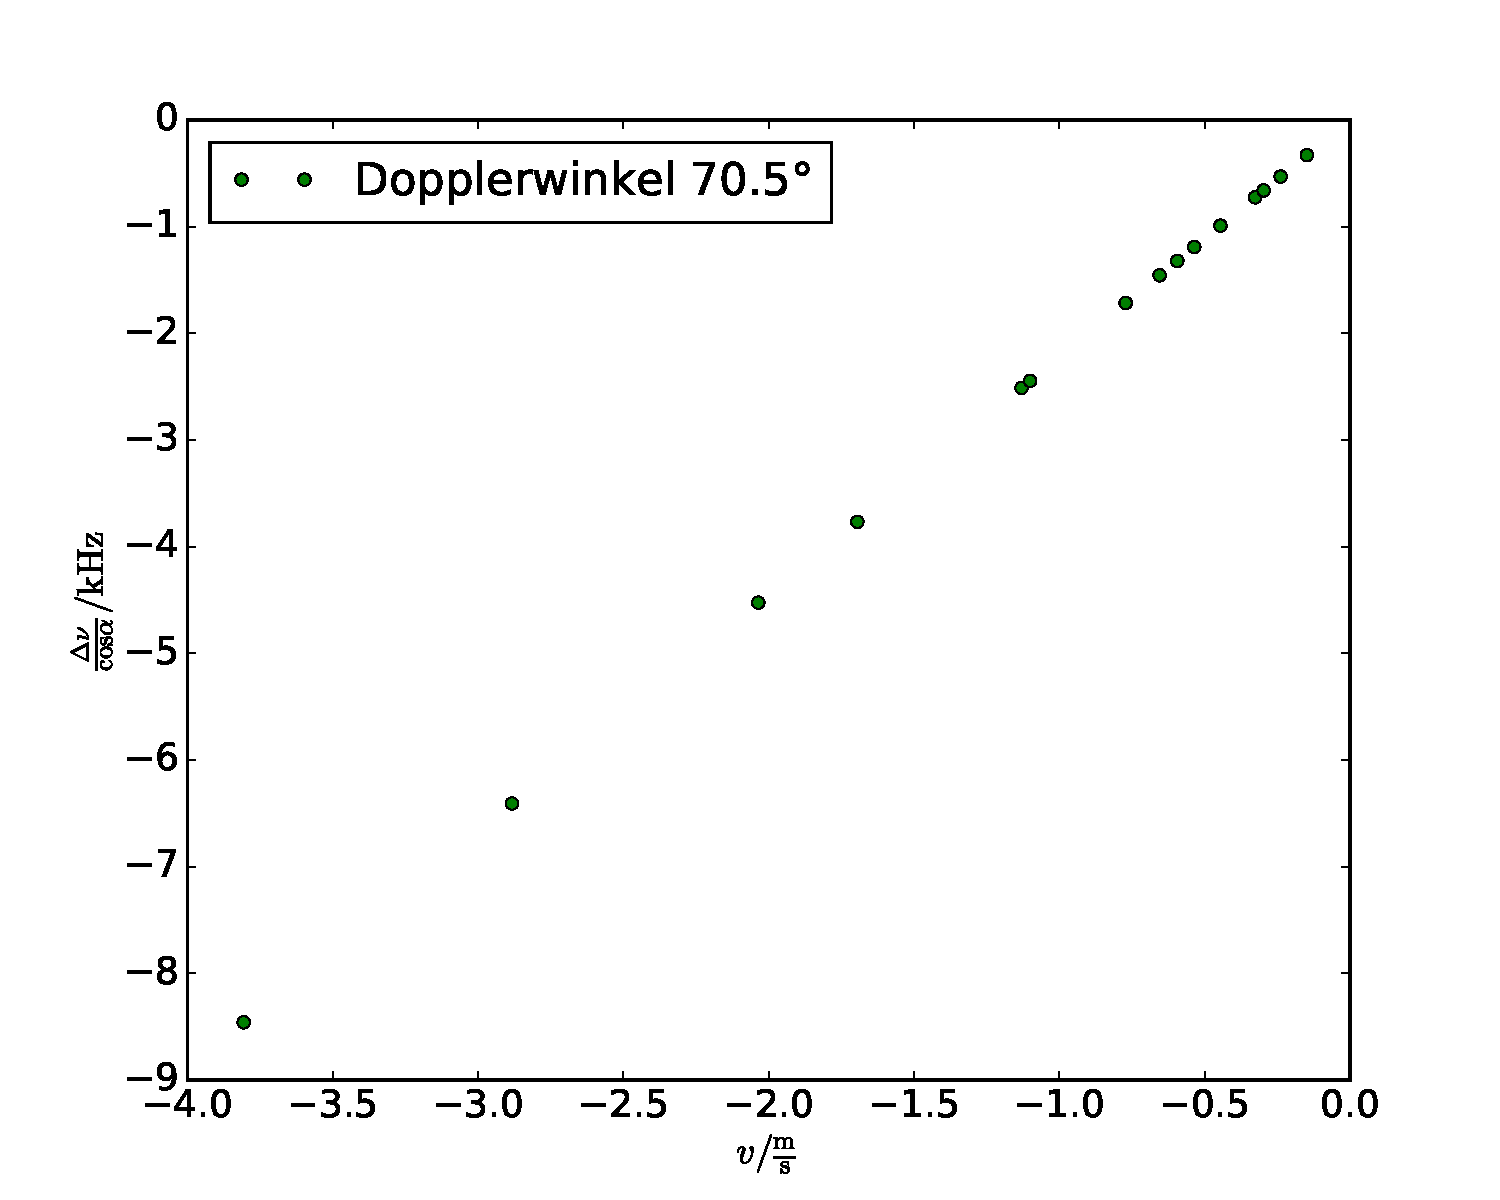
\includegraphics[width=0.8\textwidth]{a30.pdf}
        \caption{Die Frequenzverschiebung geteilt durch den cos des
        Dopplerwinkels 70.5° aufgetragen gegen die Geschwindigkeit.}
        \label{fig:2}
    \end{figure}
    \begin{table}
      \centering
      \begin{tabular}{c c c c}
        \toprule
        Pumpleistung / $\%$ & $\symup{\Delta} \nu$ / $\si{\hertz}$ & $v$ /
        \si{\meter\per\second} & Rohrdicke $\si{\milli\meter}$ \\
        \midrule
        30 & -61 & 0.15 & 16\\
        40 & -98 & 0.24 & 16\\
        50 & -134 & 0.33 & 16\\
        60 & -183 & 0.45 & 16\\
        70 & -244 & 0.59 & 16\\
        30 & -122 & 0.30 & 10\\
        40 & -220 & 0.54 & 10\\
        50 & -317 & 0.77 & 10\\
        60 & -464 & 1.13 & 10\\
        70 & -696 & 1.70 & 10\\
        30 & -269 & 0.66 & 7\\
        40 & -452 & 1.10 & 7\\
        50 & -836 & 2.04 & 7\\
        60 & -1184 & 2.88 & 7\\
        70 & -1563 & 3.81 & 7\\
      \bottomrule
      \end{tabular}
      \caption{Die Pumpleistung, die Frequenzverschiebung (aus den Messungen)
      und die Geschwindigkeit aus \eqref{eqn:geschw} berechnet für einen
      Einfallswinkel von 30°.}
      \label{tab:3}
    \end{table}

      \begin{figure}
        \centering
          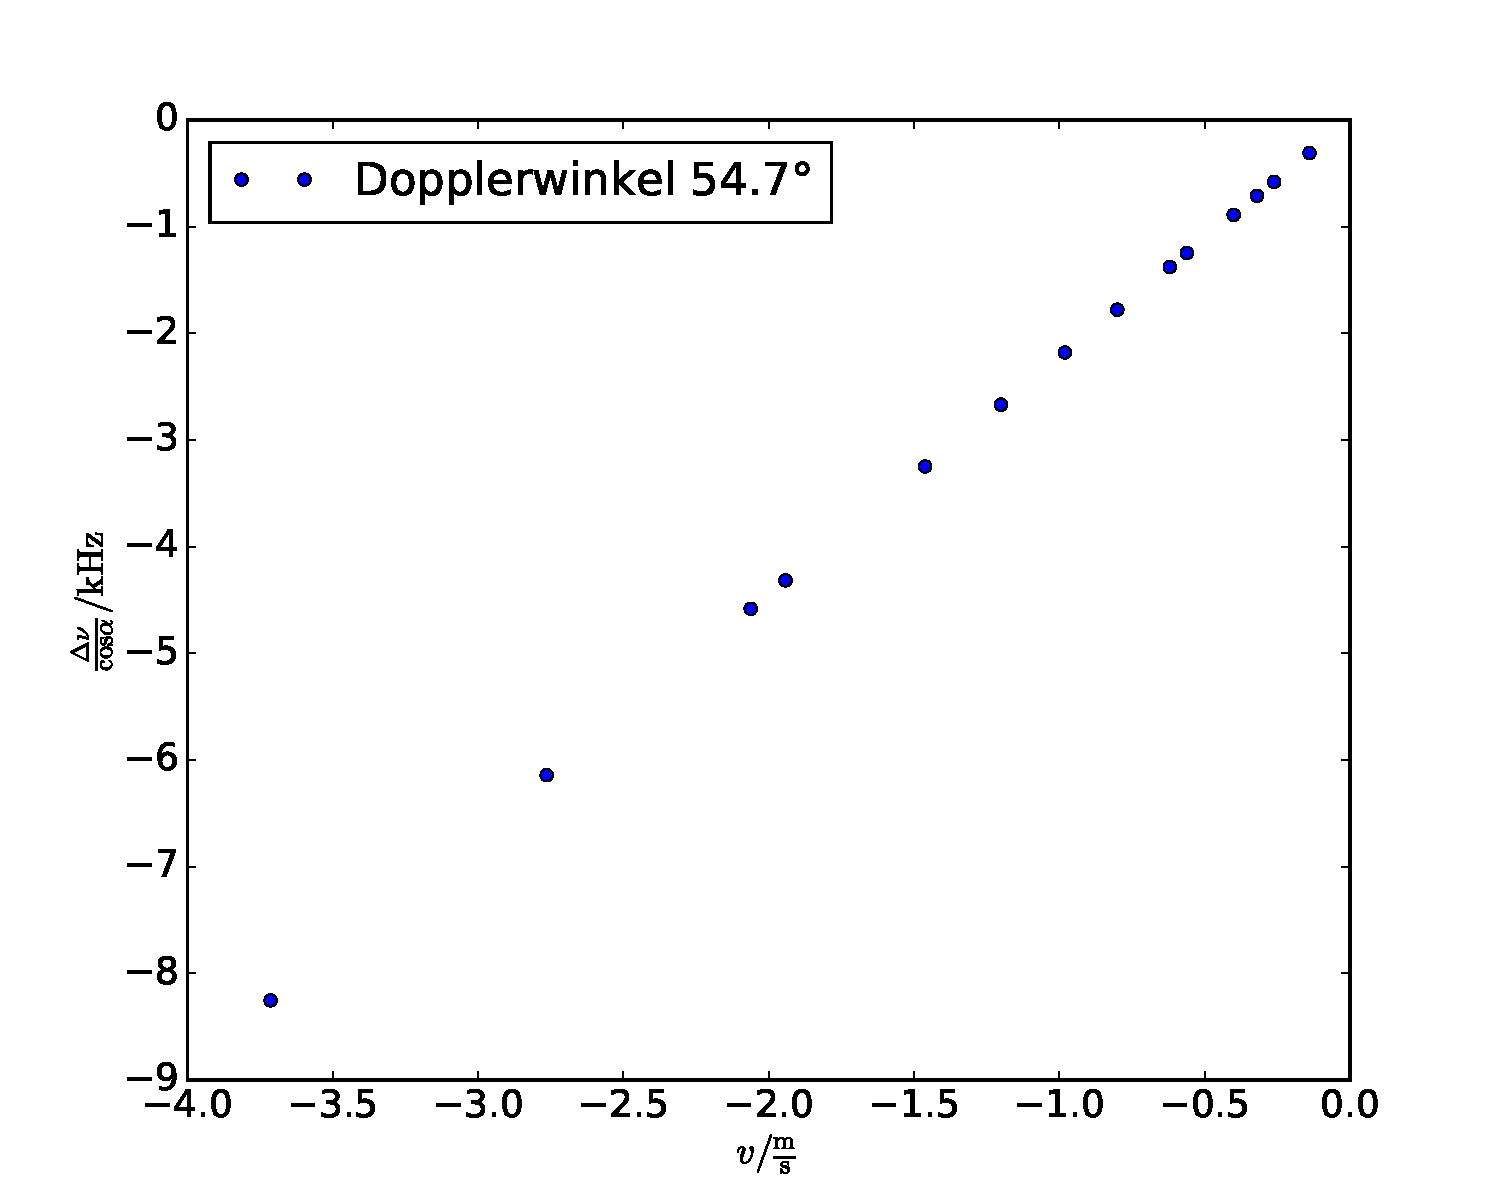
\includegraphics[width=0.8\textwidth]{a60.pdf}
          \caption{Die Frequenzverschiebung geteilt durch den cos des
          Dopplerwinkels 54.7° aufgetragen gegen die Geschwindigkeit.}
          \label{fig:3}
      \end{figure}

      \begin{table}
        \centering
        \begin{tabular}{c c c c}
          \toprule
          Pumpleistung / $\%$ & $\symup{\Delta} \nu$ / $\si{\hertz}$ & $v$ /
          \si{\meter\per\second} & Rohrdicke $\si{\milli\meter}$ \\
          \midrule
          30 & 85 & 0.14 & 16\\
          40 & 159 & 0.26 & 16\\
          50 & 244 & 0.40 & 16\\
          60 & 342 & 0.56 & 16\\
          70 & 488 & 0.80 & 16\\
          30 & 195 & 0.32 & 10\\
          40 & 378 & 0.62 & 10\\
          50 & 598 & 0.98 & 10\\
          60 & 891 & 1.46 & 10\\
          70 & 1184 & 1.94 & 10\\
          30 & 342 & 0.56 & 7\\
          40 & 732 & 1.20 & 7\\
          50 & 1257 & 2.06 & 7\\
          60 & 1685 & 2.76 & 7\\
          70 & 2264 & 3.71 & 7\\
          \bottomrule
        \end{tabular}
        \caption{Die Pumpleistung, die Frequenzverschiebung (aus den Messungen)
        und die Geschwindigkeit aus \eqref{eqn:geschw} berechnet für einen
        Einfallswinkel von 60°.}
        \label{tab:4}
      \end{table}


    \subsection{Bestimmung der Streuintensität und der Momentangeschwindigkeit
    in
      Abhängigkeit von der Messtiefe}
      Zur Bestimmung der Momentangeschwindigkeit wird \eqref{eqn:freqdiff} genutzt mit
      $\alpha = 80.1°$ und dem gemessenen Wert für $\symup{\Delta} \nu$. Für
      $\nu_0$
      wird $\SI{2}{\mega\hertz}$ und für $c$
      $\SI{1800}{\meter\per\second}$ verwendet. Für die Messtiefe wird die
      Umrechnung
         $4 \, \symup{\mu s} = 6 \, \symup{mm}$
      verwendet. Im Folgenden sind die Ergebnisse als
      Tabelle und Diagramm aufgelistet.

      \begin{figure}
        \centering
        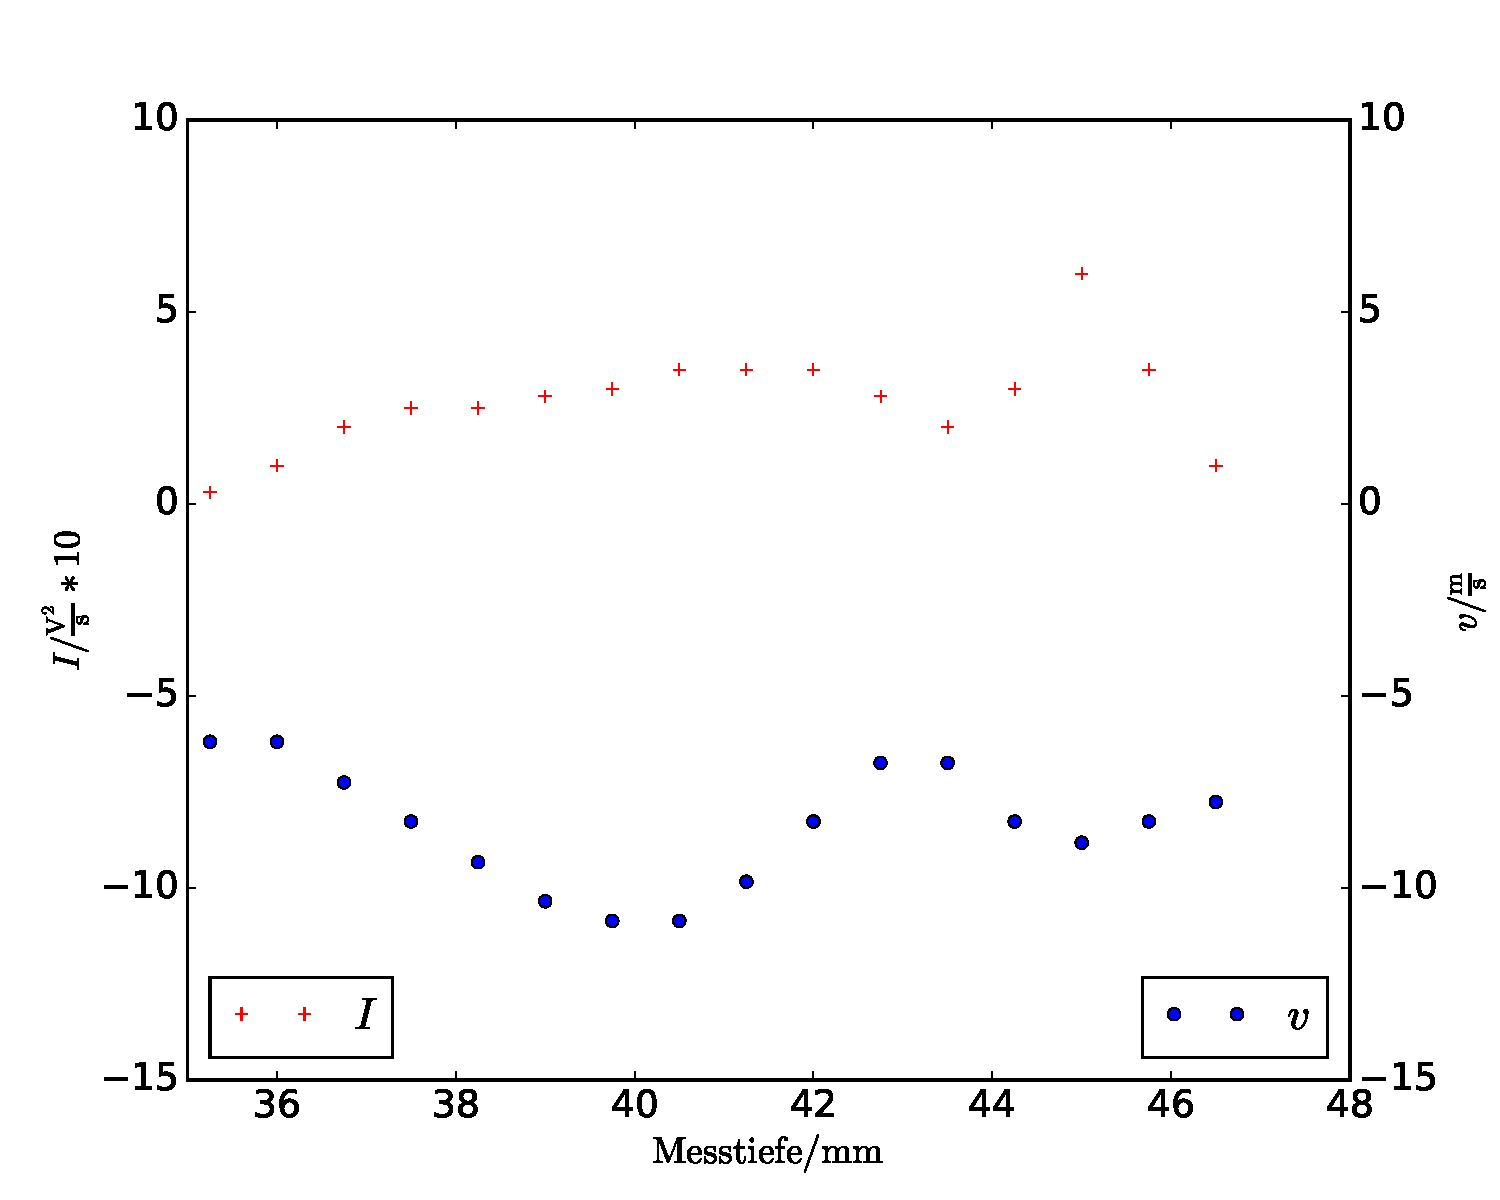
\includegraphics[width=0.8\textwidth]{b45.pdf}
        \caption{Momentangeschwindigkeit und Streuintensität in Abhängigkeit
        von der Messtiefe aufgetragen.}
        \label{fig:4}
      \end{figure}
      \begin{table}
        \centering
        \begin{tabular}{c c c}
            \toprule
            Messtiefe / $\si{\meter\meter}$ & $v$ / $\si{\meter\per\second}$ &
            $I$ / $\si{\volt\squared\per\second} \cdot 1000$ \\
            \midrule
            30 & 6.19 & 30 \\
            30.75 &  6.19 & 100 \\
            31.5 & 7.25 & 200 \\
            32.25 & 8.27 & 250 \\
            33 & 9.33 & 250 \\
            33.75 &  10.35 & 280 \\
            34.5 & 10.86 & 300 \\
            35.25 & 10.86 & 350 \\
            36 & 9.84 & 350 \\
            36.75 & 8.27 & 350 \\
            37.5 & 6.74 & 280 \\
            38.25 & 6.74 & 200 \\
            39 & 8.27 & 300 \\
            39.75 & 8.82 & 600 \\
            40.5 & 8.27 & 350 \\
            41.25 & 7.76 & 100 \\
            \bottomrule
        \end{tabular}
        \caption{Messtiefe, Momentangeschwindigkeit $v$ und Streuintensität $I$.}
        \label{tab:5}
      \end{table}

      \begin{figure}
        \centering
        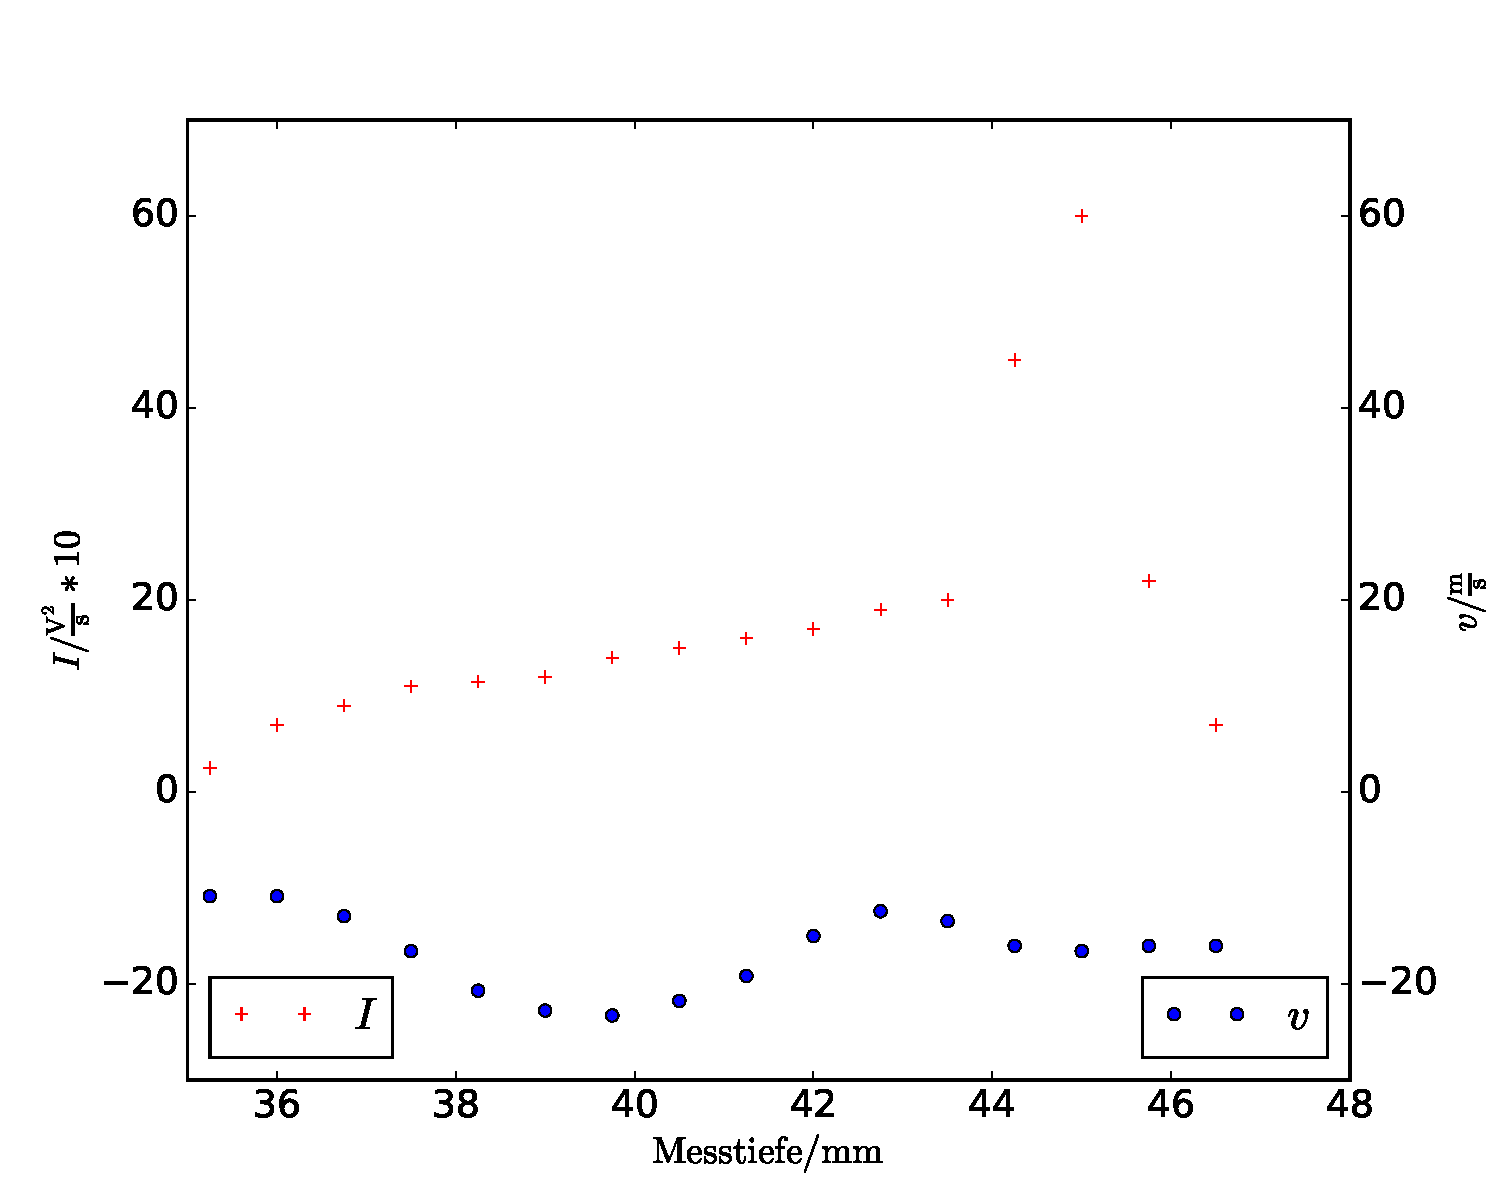
\includegraphics[width=0.8\textwidth]{b70.pdf}
        \caption{Momentangeschwindigkeit und Streuintensität in Abhängigkeit
        von der Messtiefe aufgetragen.}
        \label{fig:5}
      \end{figure}
      \begin{table}
        \centering
        \begin{tabular}{c c c}
          \toprule
          Messtiefe / $\si{\meter\meter}$ & $v$ / $\si{\meter\per\second}$ &
          $I$ / $\si{\volt\squared\per\second} \cdot 1000$ \\
          \midrule
          30 & 10.86 & 250 \\
          30.75 & 10.86 & 700 \\
          31.5 & 12.93 & 900 \\
          32.25 & 16.58 & 1100 \\
          33 & 20.69 & 1150 \\
          33.75 & 22.77 & 1200 \\
          34.5 & 23.28 & 1400 \\
          35.25 & 21.75 & 1500 \\
          36 & 19.17 & 1600 \\
          36.75 & 15.01 & 1700 \\
          37.5 & 12.42 & 1900 \\
          38.25 & 13.44 & 2000 \\
          39 & 16.03 & 4500 \\
          39.75 & 16.60 & 6000 \\
          40.5 & 16.03 & 2200 \\
          41.25 & 16.03 & 700 \\
          \bottomrule
        \end{tabular}
        \caption{Messtiefe, Momentangeschwindigkeit $v$ und Streuintensität $I$.}
        \label{tab:6}
      \end{table}

\section{Diskussion}
Aus den Diagrammen \ref{fig:1} bis \ref{fig:3} folgt, dass ein linearer
Zusammenhang
zwischen dem Verhältnis aus Frequenzverschiebung und dem Cosinus des
Dopplerwinkels und
der Strömungsgeschwindigkeit vorliegt. Außerdem stimmen die
Strömungsgeschwindigkeiten bei
den Einstrahlwinkeln 30° und 60° mit einer maximalen Abweichung von
\SI{0.33}{\meter\per\second}
gut überein. Die Werte für den Einstrahlwinkel von 15° weichen etwas stärker
ab. Hier liegt die
maximale Abweichung bei \SI{0.48}{\meter\per\second} im Vergleich zu der
Messung bei 30°
bzw. bei \SI{0.50}{\meter\per\second} unter einem Winkel von 60°.\\
\\ 2: linear bis 44, danach Ausschlag, weil rohr zuende und damit störungen reinkommen
Aus Abbildung \ref{fig:4} lässt sich erkennen, dass die Geschwindigkeit zum
Rand des Rohrs hin relativ
konstant ist, während sie in der Mitte des Rohrs ein Minimum hat, was dem
Modell widerspricht.
Ähnliches gilt für Abbildung \ref{fig:5}. Es wird weiterhin ein Minimum zur Rohrmitte hin aufgewiesen.
Die Streuintensität in Abbildung \ref{fig:4} hat einen antiproportionalen Zusammenhang zur Geschwindigkeit. Die Streuintensität in Abbildung \ref{fig:5} verläuft bis zu einer Messtiefe von \SI{44}{\milli\meter} linear. Danach gibt es einen Ausschlag, weil das Rohr zuende ist und damit Störungen die Messung beeinflussen.
Möglich dafür ist hier eine Blockade des Flüssigkeitsstroms durch Knicke in den nicht
starren Kurvenstücken.
Außerdem lässt sich sagen, dass sich das Ablesen der vom Computer angezeigten
Werte bei beiden Versuchsteilen
als schwierig gestaltet hat, da sich die Werte teilweise im Sekundenintervall
änderten.
Dadurch sind systematische Fehler nicht auszuschließen. Abschließend lässt sich
feststellen,
dass der erste Teil des Versuchs gute Ergebnisse geliefert hat, während der
zweite Teil mit einigen systematischen Fehlern belastet ist.
\newpage
\nocite{*}
\printbibliography
\end{document}
